\documentclass{article}
\usepackage{graphicx}
\usepackage{listings}
\usepackage{flexisym}
\usepackage{graphicx}

\begin{document}

  \title{ECE 375: Assignment 1}
  \author{Jared Wasinger}

  \maketitle

  \begin{enumerate}
      \item Suppose a processor or CPU supports 64 different instructions and has a memory of 1K (K = 1024) words.
      Determine the size of each memory word for the following instruction formats:

      \begin{enumerate}
        \item\begin{enumerate}
          \item 3-address instruction format:\\
            $Opcode = 2^6 = 6 bits$\\
            $Address = 2^{10} = 10 bits$\\
            Address bits * 3 + Opcode bits = 36 bits
          \item 2-address instruction format:\\
            $Opcode = 2^6 = 6 bits$\\
            $Address = 2^{10} = 10 bits$\\
            Address bits * 2 + Opcode bits = 26 bits
          \item 1-address instruction format:\\
            $Opcode = 2^6 = 6 bits$\\
            $Address = 2^{10} = 10 bits$\\
            Address bits * 1 + Opcode bits = 16 bits
        \end{enumerate}
        \item The advantage of a three-address instruction format vs a 2-address one is that it allows a wider variety of types of instructions.  For example, if I wanted an instruction that could add two registers and store the results in a third, I could conceivably do this with one expression.\\
        However in a two address instruction format, this same operation would take more instructions.  In order to perform addition and then move the result to a target register, the addition command would have to be invoked, then the result moved from the hardcoded output register of said command to the target register.\\

        The downside of a three-address instruction format is that it makes each instruction take up more memory than a two-address format.  This would limit the total amount of instructions that a program could use and would potentially be severely limiting.\\
      \end{enumerate}
    \item 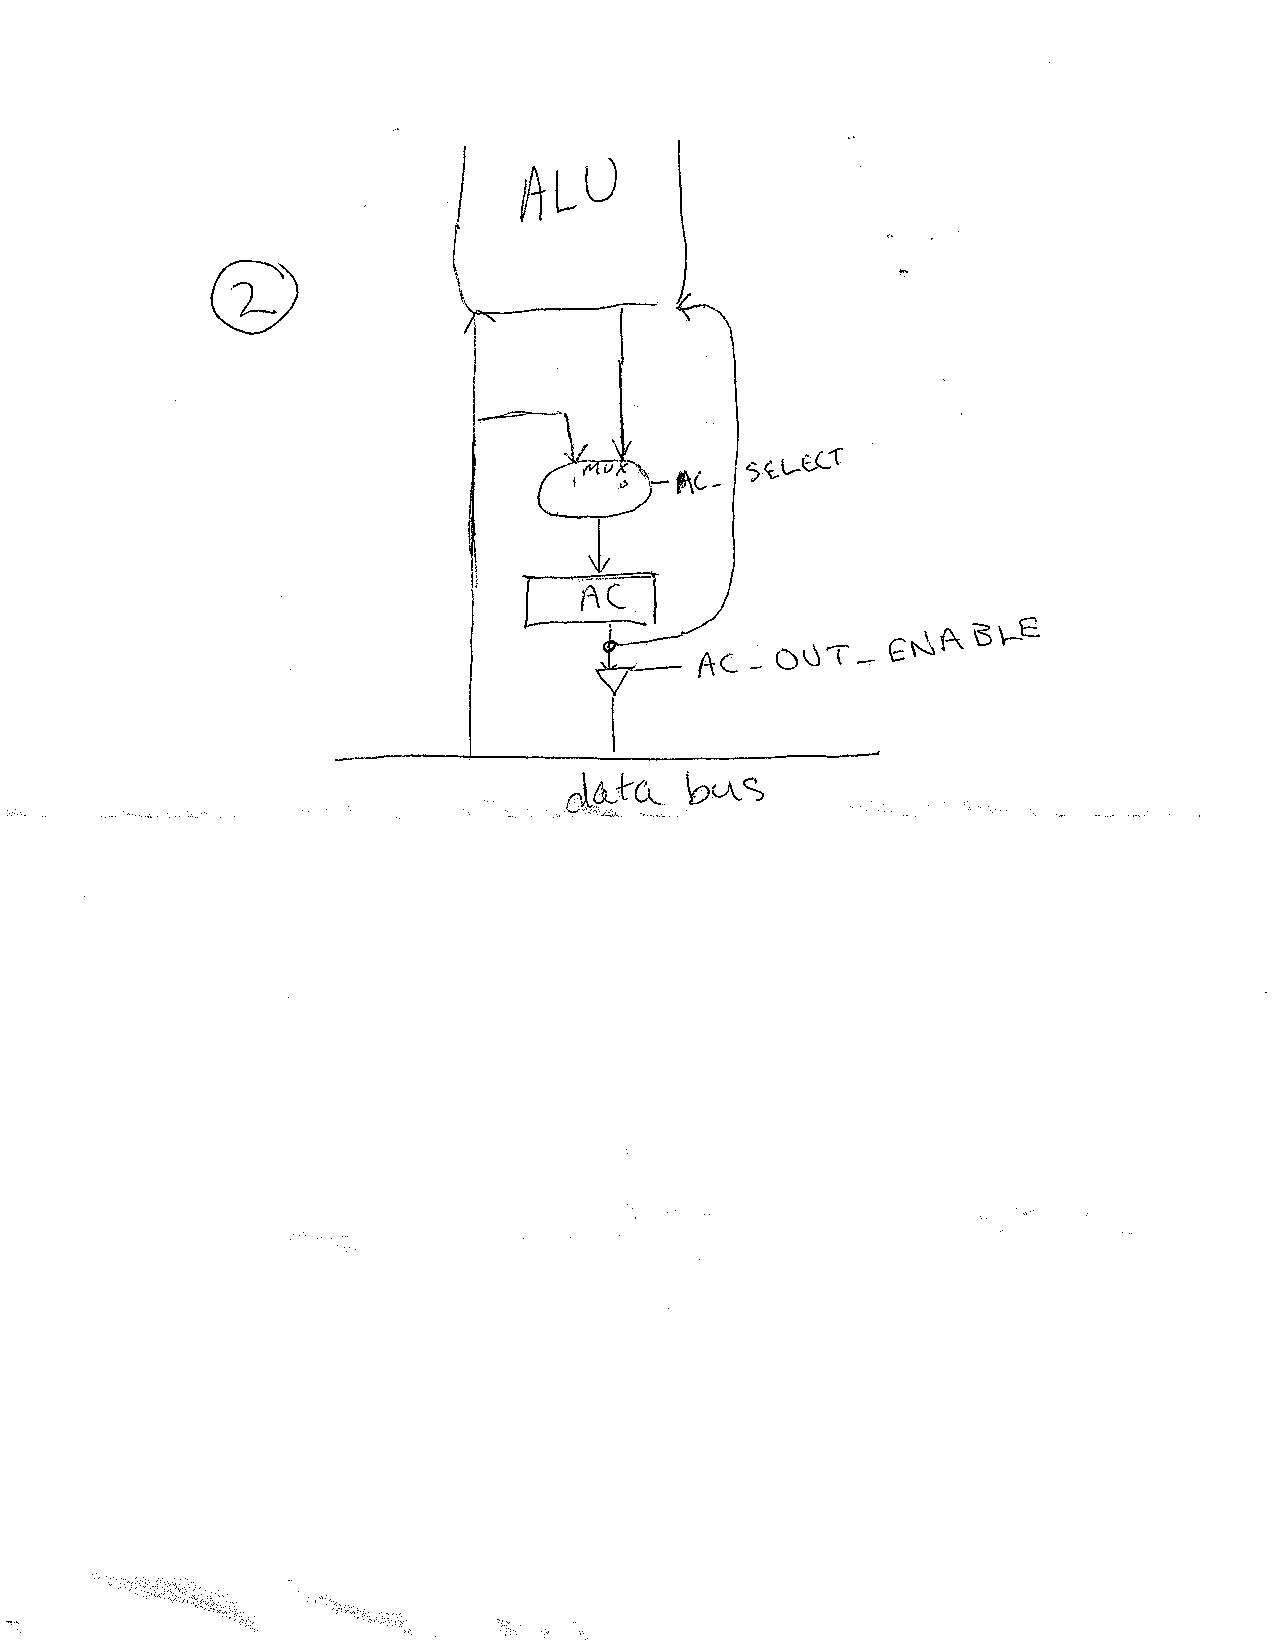
\includegraphics{a1-p2.jpg}
    \item\begin{enumerate}
      \item This is not possible because AC and MAR would have to travel across the bus simultaneously.
      \item $IR \leftarrow MDR, MAR \leftarrow MDR$\\
        This is possible as long as the number of bits being sent is specified.  becuase $IR_size \textless MDR_size$ and $MAR_size < MDR_size$.
      \item $MAR \leftarrow MDR, MDR \leftarrow M(MAR)$
        This is possible because $MAR$ will have a value and thus, does not depend on $MAR \leftarrow MDR$ to get the address that needs to be retrieved from.
      \item $MDR \leftarrow AC + 1$
        Not possible: $AC+1$ will take one step, and it will take another for $MDR$ to receive the value.
      \item $AC \leftarrow MDR, PC \leftarrow PC + 1$
        Possible: PC can perform the addition using internal adder without sending anythin across the bus.
      \item $PC \leftarrow PC + AC$
        Not possible:  This operation would take two cycles and more steps.  First the value from PC must sent to AC over the bus.  Then the addition must be performed and sent back to PC.
    \end{enumerate}
    \item $STA^{-}: M(x) \leftarrow M(x) - 1, M(M(x)) \leftarrow AC$
    \begin{enumerate}
      \item $MAR \leftarrow X, TEMP \leftarrow AC$
      \item $MAR \leftarrow MDR, AC \leftarrow MDR$\\
      Get $M(M(x))$ and store $M(X)$ in $AC$.
      \item $MDR \leftarrow TEMP$
      Store old $AC$ in $M(M(x))$, and decrement current AC (holding $M(x)$)
      \item $AC \leftarrow AC - 1$
      \item ....
    \end{enumerate}
    \item\begin{enumerate}
      \item $X \leftarrow X -2, X = 0104$
      \item $X_{H} \leftarrow 85, X = 8506$
      \item $0x1B = 0b 0001 1011 -> $Rotate right through carry$ -> 0b 1000 1101; r2 = 0b10001101$
      \item $r2 + r1 + C = 0x1B + 0x05 + 0x1 = 0x22; r2 = 0x22$
      \item $M(0x0007) \leftarrow r28 = M(0x0007 \leftarrow X_L = M(0x0007)$; The registers and memory locations shown do not change.
    \end{enumerate}
  \end{enumerate}
\end{document}
